%TODO criteria bekijken

\chapter{Vergelijkingscriteria}
\label{chap:vergelijkingscriteria}

Dit hoofdstuk bekijkt hoe de mobiele HTML5 raamwerken zullen worden vergeleken.
Hoofdzakelijk zal dit gebeuren aan de hand van een \term{proof of concept}~(POC).
Deze wordt geïntroduceerd in sectie \ref{sec:vergelijking-poc} en zal hoofdzakelijk de gekozen vergelijkingscriteria in sectie \ref{sec:vergelijking-criteria} drijven.
De criteria die worden voorgesteld, zullen voortaan actieve criteria worden genoemd.


\section{POC}
\label{sec:vergelijking-poc}
In sectie \ref{sec:vergelijking-poc-idee} wordt het idee van de gekozen POC besproken, waarna in sectie \ref{sec:vergelijking-poc-detail} de fases die door een werknemer worden uitgevoerd, gedetailleerd worden besproken.

\subsection{Idee}
\label{sec:vergelijking-poc-idee}

In samenspraak met Capgemini werd gekozen om een \term{proof of concept}~(POC) op te stellen.
Dit is een idee waarbij de uitvoerbaarheid in de verschillende raamwerken kan worden nagegaan.
Verschillende vergaderingen werden georganiseerd om tot een idee te komen dat vooral in de bedrijfswereld van toepassing is.
Het uiteindelijke idee is een applicatie die het mogelijk maakt voor werknemers om hun onkosten via hun mobiel apparaat door te sturen.

Het idee werd uitgewerkt door Capgemini en geleverd aan de auteurs als \term{mockup}.
Dit is een voorstelling van de applicatie als een reeks schermen zoals deze er zouden uitzien op een apparaat. 
Een voorbeeld van zo een scherm is te vinden op figuur~\ref{fig:poc}. 
De bedoeling is dat deze POC wordt uitgewerkt zowel voor smartphone als tablet, zowel voor Android als iOS, zowel voor staande als liggende apparaten en zowel voor online als offline gebruik.

\begin{figure}
  \centering
  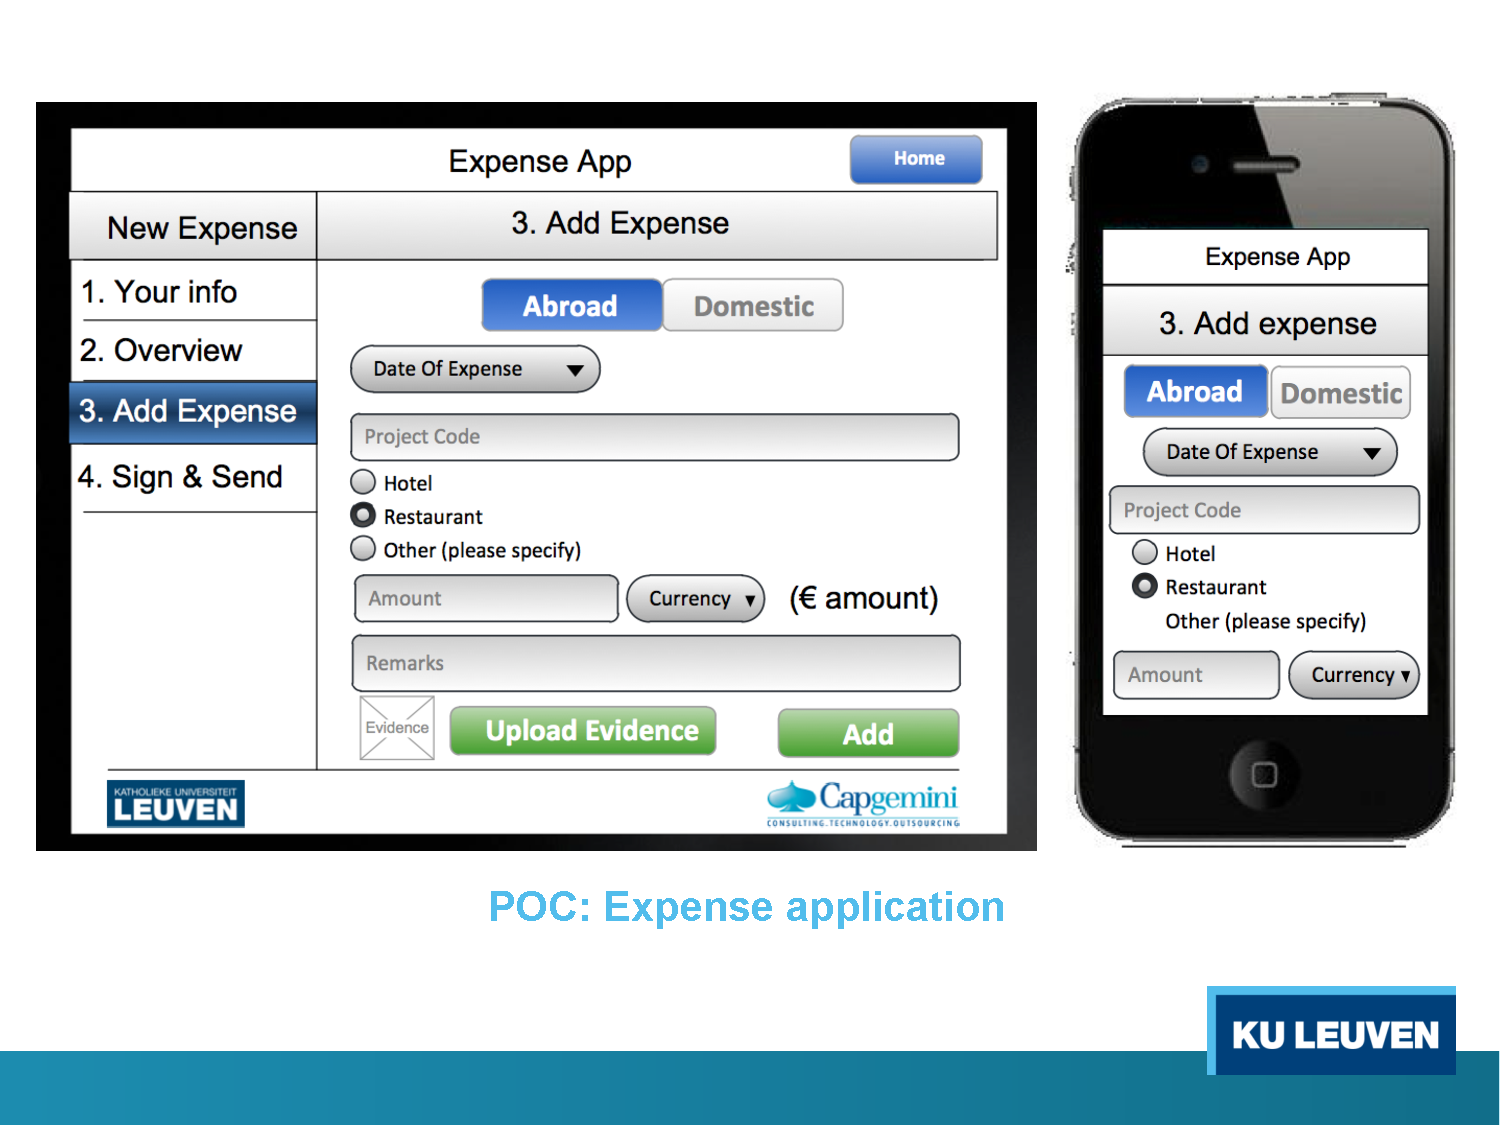
\includegraphics[trim=0cm 4cm 0cm 1.25cm,clip=true,height=7.5cm]{figuren/poc.pdf}
  \caption{POC bij het toevoegen van een nieuwe onkost met aan de linkerkant de weergave op een tablet en aan de rechterkant deze op een smartphone.}
  \label{fig:poc}
\end{figure}

\subsection{Aspecten}
\label{sec:vergelijking-poc-detail}

Een werknemer meldt zich eerst aan op de applicatie en kan daarna ofwel een nieuw onkostenformulier aanmaken of zijn doorgestuurde onkostenformulieren bekijken.
De term onkostenformulier is een groepering van meerdere onkosten met bijhorende bewijsstukken en de handtekening van de werknemer. 
Het aanmaken van een nieuw onkostenformulier verloopt in vier stappen.
Indien de werknemer al eerder begonnen was met het aanmaken van een formulier, zal hij worden gevraagd of hij verder wil gaan met dat formulier of met een nieuw formulier wil starten.

%TODO Ik kreeg het gevoel dat de schrijfstijl veranderd.  Soms wordt er naar 'zijn', 'hij', ... verwezen,  dan weer is er de beschrijvende stijl met een verwijzing naar 'de werknemer`.. snapte? :) Tim: nee

\begin{enumerate}
\item De eerste stap is het bekijken en/of aanpassen van de persoonlijke informatie van de werknemer.
Bij het aanpassen van deze gegevens, zullen deze worden gevalideerd.
Indien deze validatie faalt, krijg de werknemer een dialoogvenster te zien met de reden tot falen.
Ook worden de foute velden rood gemarkeerd.

\item In de tweede stap kan de werknemer zijn toegevoegde onkosten aan het formulier bekijken.
In het begin is deze lijst leeg, tenzij hij eerder een formulier aan het invullen was (zie infra).
Indien deze lijst onkosten bevat, is het mogelijk om hierop te klikken en deze te bekijken. Aanpassen is niet mogelijk.

\item In stap drie kan een nieuwe onkost worden toegevoegd.
Dit kan ofwel een binnenlandse ofwel buitenlandse onkost zijn.
Voor beide dient een datum en projectcode te worden opgegeven.
De eerstgenoemde is een \term{datepicker} die teruggaat tot twee maanden in de tijd.
De laatstgenoemde bevat automatische aanvulling, maar de werknemer is niet verplicht om een projectcode uit de aanvulling te selecteren.
Daarnaast dient het type en bedrag van de onkost, alsook een bewijsstuk te worden opgegeven.
Bij een buitenlands onkost moet de munteenheid worden opgegeven, waarna de applicatie deze automatisch omvormt naar euro.
Het scherm voor het toevoegen van een buitenlandse onkost wordt getoond op figuur \ref{fig:poc}. 
Net zoals bij stap één geldt ook hier validatie op de formuliervelden.

\item In deze laatste stap dient een handtekening te worden geplaatst waarna het formulier kan worden doorgestuurd.
Indien de gebruiker offline werkt, zal deze worden opgeslagen op het toestel.
De werknemer kan het formulier opnieuw doorsturen zodra hij terug online is.

\end{enumerate}

Bij het bekijken van de doorgestuurde formulieren is het mogelijk om per formulier de bijhorende PDF te downloaden. 
Deze bevat een overzicht van de onkosten met bijhorende bewijsstukken, alsook de handtekening van de werknemer.

\section{Criteria}
\label{sec:vergelijking-criteria}

In deze sectie zullen de actieve criteria toelicht worden die zullen worden toegepast om de raamwerken te vergelijken.
In sectie \ref{sec:vergelijken-raamwerken} werden reeds technieken besproken die in de literatuur worden toegepast.
Elementen van deze technieken zullen terugkomen in onze methode om de raamwerken te evalueren.
Sectie \ref{sec:raamwerken-tabel} bevatte de passieve vergelijkingscriteria die raamwerken vergeleken met informatie van het raamwerk zelf.

Vijf grote criteria zullen worden gebruikt: populariteit (\ref{sec:vergelijking-populariteit}), productiviteit (\ref{sec:vergelijking-productiviteit}), gebruik (\ref{sec:vergelijking-gebruik}), ondersteuning (\ref{sec:vergelijking-ondersteuning}) en performantie (\ref{sec:vergelijking-performantie}). 
Elk raamwerk krijgt voor elk criterium een score. 
Deze scores zullen in een spinnenweb worden ondergebracht (zie sectie \ref{sec:vergelijking-spinnenweb}).
Zoals hierboven vermeld zal een POC gebruikt worden bij de vergelijking.
De implementatie van deze POC zal het productiviteits-, gebruiks- en ondersteuningscriterium drijven.  
Dit komt omdat Capgemini de POC zo heeft opgesteld dat het verschillende functionaliteit bevat om een volledige vergelijking te kunnen maken.

De score van performantie zal deels bepaald worden door de laadtijden van de POC.

\subsection{Populariteit}
\label{sec:vergelijking-populariteit}
De populariteit van een raamwerk is in cijfers uit te drukken door gebruik te maken van sociale netwerken. 
Een tabel zal voorzien worden met in de kolommen het aantal volgers op Twitter, sterren en forkers van GitHub,  vragen op Stackoverflow en aantal vind-ik-leuks van Facebook en de raamwerken in de rijen~\cite{Sarrafi2012a,Ayuso2012}. 

GitHub kan worden gezien als exacte weergave van de actieve gemeenschap rond het raamwerk. %TODO referentie?
Zowel \st{} als \kendo{} echter, zijn niet op GitHub terug te vinden.
Hierdoor zal de score voor sterren en forkers van GitHub voor beide raamwerken gelijk zijn aan nul.
Een alternatief hield de interpolatie van de GitHub data van de overige raamwerken in.
Omdat deze aanpak het raamwerk onterecht zou bevoordelen, is hier niet voor gekozen.

De som van Twitter volgers ($T_r$), GitHub sterren ($S_r$), GitHub forkers ($F_r$), Stackoverflow vragen ($SO_r$) en Facebook vind-ik-leuks ($FB_r$) vormt de score voor het gemeenschapscriteria:
\begin{equation}
  GM_r=T_r+S_r+F_r+SO_r+FB_r
  \label{eq:populariteit}
\end{equation}
met $r$ de verschillende raamwerken.

De uitkomsten van dit criterium zullen vergeleken worden met data geleverd door Google Trends. %TODO referentie
Deze applicatie toont de evolutie van zoektermen op Google
Voor elk raamwerk zal het volume zoekopdrachten naar het raamwerk in functie van de tijd worden uitgezet.
%TODO bekijken evolutie van data in de tijd?

\paragraph{Motivatie}

Er bestaat geen exacte formule om populariteit uit te drukken.
De formule die werd gekozen om de score voor dit criterium te quoteren is onderheven aan subjectiviteit.
Twee opmerkingen moeten hierbij worden gemaakt.
Enerzijds zijn de auteurs zich ervan bewust dat de doorsnede tussen sociale netwerken niet leeg is.
Zo kan éénzelfde persoon zowel een volger op Twitter zijn als fan op Facebook.
Verschillende individuen zullen dus dubbel geteld worden in de totale score voor populariteit van het raamwerk.
De score zal dus slechts een indicatie geven over de popularieit,  het is geen exacte weergave.
Ten tweede zijn de auteurs er zicht van bewust dat de inclusie van Stackoverflow op twee manieren kan worden bekeken.
Enerzijds kunnen veel vragen over één onderwerp op Stackoverflow duiden op veel vraagtekens over dit onderwerp.
Anderzijds kan dit een maat zijn voor de populariteit van dit onderwerp.
De auteurs zijn van mening dat de tweede zienswijze correcter is dan de eerste en het dus valied is Stackoverflow in de formule op te nemen.

%%%%%%%%%%%%%%%%%%%%%%%%%%%%%%%%%%%%%%%%%%%%%%%%%%%%%%%%%%%%%%%%%%
%%%%%%%%%%%%%%%%%%%%%%%%%%%%%%%%%%%%%%%%%%%%%%%%%%%%%%%%%%%%%%%%%%

\subsection{Productiviteit}
\label{sec:vergelijking-productiviteit}
De productiviteit moet een indicatie geven hoe lang het duurt om met het raamwerk vertrouwd te raken.
De auteurs zullen het raamwerk testen met een implementatie van de POC.
Er kan verondersteld worden dat de auteurs over een gemeenschappelijke technische achtergrond beschikken.

Elk zullen ze de POC in twee verschillende raamwerken maken,  daarnaast ook een extra login applicatie in twee andere raamwerken.
Tim Ameye maakt de POC in \jqm{} en \lungo{} en de login applicatie in \st{} en \kendo{}.
Sander Van Loock zal dan de POC in \st{} en \kendo{} maken en de login applicaties in \jqm{} en \lungo{}.
De tijd die nodig is om de volledige POC te implementeren is een indicatie voor de productiviteit. 
De implementatie van de login applicatie is een extra test.
Deze applicatie bevat GI-elementen, validaties,  \term{backend} integratie en lijsten.
Deze test kan dit dus als voldoende steekproef beschouwd worden om ervaring met een raamwerk te testen.
Na het aanmelden met deze applicatie zal de gebruiker een lijst van $850$ elementen te zien krijgen.
Deze lijst is voornamelijk bedoeld om de performantie te testen (zie sectie \ref{sec:vergelijking-performantie}).
De elementen in de lijst zullen voorzien worden van een afbeelding en tekst.
Het aantal elementen in de lijst - $850$ - is een schatting van het aantal liedjes die Elvis Presley ooit heeft opgenomen. %TODO referentie
Deze keuze werd gemaakt met het oog op potentiele muziek applicaties die alle nummers van een artiest ook in lijsten samenbrengt.
Elvis Presley is de artiest die het meeste opgenomen nummers achter zijn naam heeft staan en kan dus als bovengrens voor dit soort applicaties worden beschouwd.
De implementatie van deze applicatie zal een indicatie geven hoe snel,  zonder al te veel voorkennis van het raamwerk,  één eenvoudige applicatie opgeleverd kan worden.
De tijd die ieder nodig heeft om deze applicatie te bouwen, geeft dus een indicatie van de nodige leertijd.


De som van de uren voor het implementeren van de POC ($t_{r,POC}$) en de login applicatie ($t_{r,login}$) vormt de score voor de productiviteit:
\begin{equation}
  PR_r = {t_{r,POC} + t_{r,login}}
  \label{eq:productiviteit}
\end{equation}
waar $r$ de verschillende raamwerken voorstellen.

De uitkomsten van dit criterium zullen gestaafd worden met zes argumenten.
Eerst zullen het aantal tools bekeken worden die de programmeur kan gebruiken om eenvoudiger te ontwikkelen.
Ook zullen de factoren die de leercurve bepalen, worden geschat.
Vervolgens zal de kwaliteit en quantiteit van de documentatie van elk raamwerk worden bekekenen.
De mogelijkheden voor debuggen bepalen ook de productiviteit en zullen bekeken worden.
Tot slot zal gekeken worden naar de aanwezige literatuur van het raamwerk en waar ontwikkelaars met vragen terecht kunnen.

% \newcounter{assumpties}
% \begin{enumerate}[\textbf{Item} i]
%   \item \label{ass:poc} De POC bevat alle relevate kenmerken om het raamwerk te testen voor applicaties binnen een bedrijfscontext.
%   \suspend{enumerate}
% \end{enumerate}
% 
% \begin{enumerate}[{[\textbf{Item} i]}]
%   \setcounter{assumpties}{\value{enumi}}
%   \item \label{ass:achtergrond} Beide auteurs beschikken over een gemeenschappelijke technische achtergrond.
% \end{enumerate}

\paragraph{Motivatie}

Volgens assumptie XX bevat de POC alle belangrijke componenten om het raamwerk maximaal te testen.
De tijd die nodig is om deze applicatie te bouwen, is dus zeker een geldige waarde om de productiviteit te bepalen.
Assumptie XX laat toe om met twee verschillende personen dit criterium te testen.

Omdat éénzelfde applicatie twee keer moet worden geïmplementeerd, wordt verwacht dat de tweede implementatie sneller zal verlopen.
Dit probleem is onafwendbaar en zal bij de evalatie van de data aangehaald worden.

De uren voor de implementatie van de loginapplicatie zal de score correcter maken.

De leercurve van het raamwerk zit impliciet in de score voor de productiviteit vervat.

%%%%%%%%%%%%%%%%%%%%%%%%%%%%%%%%%%%%%%%%%%%%%%%%%%%%%%%%%%%%%%%%%%
%%%%%%%%%%%%%%%%%%%%%%%%%%%%%%%%%%%%%%%%%%%%%%%%%%%%%%%%%%%%%%%%%%

\subsection{Gebruik}
\label{sec:vergelijking-gebruik}

Deze POC kan onderverdeeld worden in verschillende deelproblemen.
Deze deelproblemen worden als uitdaging aan het raamwerk voorgelegd.
Alle uitdagingen en deeluitdagingen zijn hieronder te vinden.

%\begin{table}[H]
%\centering
\pgfplotstabletypeset[
  begin table=\begin{longtable}{p{12cm}},
  end table=\end{longtable},
  skip coltypes=true,
  col sep=comma,
  string type,
  header=true,
  columns={Uitdaging},
  columns/Uitdaging/.style={column name=\textbf{Uitdagingen}, column type={l}},  
  every head row/.style={
    before row=\toprule,
    after row=\midrule},
  every last row/.style={
    after row=\bottomrule}
]{tabellen/uitdagingen.csv}
%\caption{Uitdagingen}
%\label{tabel:uitdagingen}
%\end{table}

In totaal konden 13 uitdagingen en 38 onderuitdagingen uit de POC geëxtraheerd worden.


De wijze waarop het raamwerk de uitdaging aangaat zal tot een score voor de uitdaging leiden.
Er onderscheiden zich drie gevallen.
De hoogste score ($2$) wordt toegekend wanneer bepaalde functionaliteit reeds aangeboden wordt door het raamwerk. 
Een lagere score ($1$) betekent dat een plug-in werd gezocht.
Omdat de raamwerken verderbouwen op HTML5, zal een kenmerk van HTML5 ook als plug-in beschouwd worden.
Voor een oplijsting van de HTML5 kenmerken wordt naar sectie \ref{sec:html5-css3-js} verwezen.
Wanneer de implementatie zelf diende geschreven te worden of een hack noodzakelijk was, zal de laagste score ($0$) worden toegekend.
Ook is het mogelijk  dat de uitdaging helemaal niet werd geïmplementeerd.
Dit is mogelijk wanneer het raamwerk de functionaliteit niet ondersteund,  geen plug-in werd gevonden en niet aan een eigen implementatie werd begonnen.
Dit zal leiden tot een $0$ score.
Wanneer CSS-code werd gebruikt om de uitdaging op te lossen zal de laagste score worden toegekend.
Het gebruik van CSS3 wordt echter als kenmerk van HTML5 gezien en vervolgens met $1$ gequoteerd.

Tabel \ref{tabel:scores-uitdagingen} toont de mogelijke scores $U_{r,i}$ van raamwerk $r$ en voor uitdaging $i$.
\begin{table}[h]	
  \centering
  \begin{tabular}{ll}
    \toprule
    \textbf{Score} & \textbf{Beoordelingscriteria}\\
    \midrule
    $U_{r,i} = 2$ & Ondersteund door het raamwerk\\
    $U_{r,i} = 1$ & Een plug-in is nodig of nieuwe kenmerken van HTML5\\
    $U_{r,i} = 0$ & Eigen implementatie of hack of niet geïmplementeerd\\ 
    \bottomrule
  \end{tabular}
  \caption{Beoordeling uitdagingen gebruikscriterium}
  \label{tabel:scores-uitdagingen}
\end{table}
\begin{equation}
  GB_r = \sum_{i=1}^{38}{\left(U_{r,i}\right)}
  \label{eq:gebruik}
\end{equation}
met $r$ de verschillende raamwerken en $i$ de uitdagingen.

Omdat er $38$ onderuitdagingen zijn kan het raamwerk voor dit criterium maximaal $76$ behalen.

\paragraph{Motivatie}

Alle interessante functionaliteit die in de POC werd gebruikt, zit in een uitdaging vervat.  
Interessante functionaliteit slaat op functionaliteit die potentieel door het raamwerk kan worden ondersteund.
De POC bevat bijvoorbeeld ook een omzetting van \term{identifiers} naar hun tekstuele vorm.
Dit is geen interessante functionaliteit omdat het eigen is aan de POC zelf.
De implementatie hiervan zal uitsluitend uit \term{native} \js{}-code bestaan.

De potentiele score van een uitdaging is discreet en ligt tussen $0$ en $2$.
%Deze score moet een objectief beeld geven over hoe het raamwerk de uitdaging aangaat.
Er zijn dus slechts $3$ scores waaruit gekozen kan worden om de implementatie te beoordelen.
De motivatie hiervoor is slechts de eenvoud.
Een alternatief bestond uit $4$ scores waarbij HTML5 kenmerken een lagere score kregen in vergelijking met plug-ins.
Omdat de raamwerken afhankelijk zijn van HTML5 werd hiervoor niet gekozen.
%TODO beter uitleggen?

%%%%%%%%%%%%%%%%%%%%%%%%%%%%%%%%%%%%%%%%%%%%%%%%%%%%%%%%%%%%%%%%%%
%%%%%%%%%%%%%%%%%%%%%%%%%%%%%%%%%%%%%%%%%%%%%%%%%%%%%%%%%%%%%%%%%%

\subsection{Ondersteuning}
\label{sec:vergelijking-ondersteuning}
Dit criterium moet weergeven hoe goed het raamwerk verschillende toestellen en verschillende besturingssystemen ondersteund.
% TODO Tim: duidelijker uitleggen hoe dat zit met browser en OS, nu veel te kort tussen haakjes aangehaald
Enkel de standaard browser van het besturingssysteem (Android browser/Chrome en Safari) zal beschouwd worden.
Voor Android geldt dat vanaf versie 4.0 Chrome als standaard browser wordt gezien. %TODO referentie http://androidandme.com/2012/02/applications/goodbye-old-browser-chrome-to-become-the-standard-browser-on-android-4-0-and-above/


Een context wordt gedefinieerd als één bepaalde configuratie van toestel, besturingssysteem en browser.
In elke context zal de functionaliteit van de POC op ondersteuning worden getest met uitdagingen.
Uitdagingen die gebruikt zijn om het gebruikscriterium te testen, kunnen hier worden hergebruikt.
Aangezien sommige uitdagingen triviaal gelden voor elk apparaat zal er slechts een subset van deze uitdagingen getest worden.
Triviale uitdagingen zijn uitdagingen waarbij de implementatie in elk raamwerk enkel uit \js bestaat.
Deze uitdagingen zijn:
\begin{itemize}
 \item \uit{anatomie}
 \item \uit{laadscherm}
 \item \uit{vullen}
 \item \uit{ajax}
 \item \uit{lijsten}
\end{itemize}
Er resten dan nog $8$ uitdagingen.
Voor dit criterium worden alle onderuitdagingen verwaarloosd behalve bij \uit{formulieren} en \uit{offline}.
%De onderuitdagingen zijn te specifiek om op ondersteuning te testen.
Een uitdaging zal enkel slagen als alle onderuitdagingen ondersteund worden.
Zo kan bijvoorbeeld op een apparaat getest worden of auto-aanvullen werkt.
Uitdaging \uit{autoaanvullen} bevat als onderuitdagingen het ophalen van suggesties en het tonen van een dropdownmenu.
De werking van de uitdaging is een combinatie van beide en zal dus enkel slagen als beide worden ondersteund.
De onderuitdagingen van \uit{formulieren} en \uit{offline} kunnen wel op ondersteuning worden getest.
%TODO nog vermelden dat datepicker uitdagingen zijn samengenomen?


Het is belangrijk dat het raamwerk en niet een eigen implementatie op ondersteuning wordt getest.
Wanneer een uitdaging in het vorige criterium een $0$ behaalde, wil dit zeggen dat het raamwerk de uitdaging al niet ondersteunde.
In dit geval moet er niet op ondersteuning getest worden.
Hierdoor is het aantal uitdagingen of onderuitdagingen die getest worden afhankelijk van het raamwerk.


Deze score van een uitdaging of onderuitdaging kan $1$ of $0$ zijn.
Dit slaat op respectievelijk een vlekkeloze of problematieke uitvoering.
De maximale score die het raamwerk per context kan behalen is $13$.
In totaal zullen $8$ contexten worden gebruikt.
Deze worden in tabel \ref{tabel:toestellen-hci} weergegeven.

 \begin{table}[H]
 \centering
 \pgfplotstabletypeset[
   begin table=\begin{tabular}{l l l l},
   end table=\end{tabular},
   col sep=comma,
   header=true,
   string type,
   skip coltypes=true,
   columns={Apparaat,Soort,BS,Browser},
   columns/Apparaat/.style={column name=\textbf{Apparaat}},  
   columns/Soort/.style={column name=\textbf{Soort}},
   columns/BS/.style={column name=\textbf{BS}},
   columns/Browser/.style={column name=\textbf{Browser}},
   every head row/.style={
     before row=\toprule,
     after row=\midrule},
   every last row/.style={
     after row=\bottomrule}
 ]{tabellen/apparaten.csv}
 \caption{Beschikbare apparaten met hun besturingssysteem~(BS) en browser.}
 \label{tabel:toestellen-hci}
 \end{table}


De som van de scores van de verschillende contexten bepaalt de score van het ondersteuningscriterium:
\begin{equation}
  O_r = \sum_{c=1}^{8}{\left(\sum_{i=1}^{N}U_{r,i}\right)}
  \label{eq:ondersteuning}
\end{equation}
met $r$ de verschillende raamwerken,  $N$ het aantal geïmplementeerd uitdagingen en onderuitdagingen,  $c$ de verschillende contexten en $i$ de uitdagingen. 


Indien het raamwerk een implementatie bevat voor alle uitdagingen en onderuitdagingen kan er per context maximaal $13$ gescoord worden.
Indien alle $8$ contexten alle uitdagingen en onderuitdagingen correct weergeven zal de maximale score van $104$ behaald worden.

% Per context zal ook de marktwaarde van het toestel in rekening worden gebracht om de meest gebruikte toestellen te bevoordelen.
% De marktwaarde is afhankelijk van het besturingssysteem,  de versie van het besturingssysteem en de gebruikte mobiele browser.
% Voor de marktwaarden wordt naar tabellen \ref{tabel:marktaandeel-ios-android} en \ref{tabel:marktaandeel-browsers} verwezen.
% De formule voor de marktwaarde van een bepaalde context ziet er als volgt uit:
% %TODO Sander: ook gewicht van device?
% \begin{equation}
%   G_c = G(BS_c)*G(BS_{c,v})*G(Browser_c)
%  \label{eq:marktwaarde}
% \end{equation}
% met $G$ de functie die de marktwaarde teruggeeft.  
% De marktwaarde voor Android en iOS ($G(BS_c)$) werd vermeld in sectie \ref{sec:mobiele-besturingssystemen}.
% De relatieve marktwaarde van de versie van dat besturingssysteem ($G(BS_{c,v})$) kan gevonden worden in tabel \ref{tabel:marktaandeel-ios-android}.
% De marktwaarde van mobiele webbrowsers ($G(Browser_c)$) kan gevonden worden in tabel \ref{tabel:marktaandeel-browsers}.
% 
% In tabel \ref{tabel:toestellen-hci} staan de verschillende contexten met hun marktwaarde weergegeven.

\paragraph{Motivatie}
De keuze van de $8$ contexten waarop ondersteuning wordt getest, is voornamelijk bepaald door het beschikbaarheid van de apparaten op het departement computerwetenschappen van de KU Leuven.
Er werd een evenwichtige keuze gemaakt tussen besturingssysteem,  browser en type apparaat.
Er werd gekozen voor $4$ Android en $4$ iOS apparaten.
Bij de $4$ Android apparaten zijn er $2$ met een Android browser en $2$ met Chrome browser.
Ook werd er gekozen voor $4$ smartphones en $4$ tablets.

%%%%%%%%%%%%%%%%%%%%%%%%%%%%%%%%%%%%%%%%%%%%%%%%%%%%%%%%%%%%%%%%%%
%%%%%%%%%%%%%%%%%%%%%%%%%%%%%%%%%%%%%%%%%%%%%%%%%%%%%%%%%%%%%%%%%%

\subsection{Performantie}
\label{sec:vergelijking-performantie}
Dit criterium zal de laattijden van het raamwerk in rekening brengen.

Hier onderscheiden zich vier gevallen.
Ten eerste zal de laadtijd van de volledig geïmplementeerde POC bekeken worden ($l_{r,c,POC}$). 
Vervolgens zal de tijd worden opgemeten om de POC uit het cachegeheugen te laden ($l_{r,c,POC_{cache}}$).
Dezelfde twee gevallen zullen ook voor de loginapplicatie die in sectie \ref{sec:vergelijking-productiviteit} werden geïntroduceerd, worden opgemeten ($l_{r,c,login}$ en $l_{r,c,login_{cache}}$).
De redenen waarom deze applicatie wordt gebruikt, is omdat ervan kan worden uitgegaan dat niet de volledige POC in ieder raamwerk zal kunnen worden geïmplementeerd. 
Dit is in tegenstelling tot deze applicatie die gelijkaardig is in de vier raamwerken.
De laadtijden kunnen vervolgens objectiever vergeleken worden en het aantal lijnen code kan verschillen verklaren.

De laadtijden voor de vier gevallen zullen op acht verschillende apparaten worden opgemeten.
Dit zijn dezelfde als bij het ondersteuningscriterium (zie tabel \ref{tabel:toestellen-hci}).

De formule voor het performantiecriterium wordt dan: 

\begin{equation}
  PE_r= \sum_{c=1}^{8}{\left(l_{r,c,POC}+l_{r,c,POC_{cache}}+l_{r,c,login}+l_{r,c,login_{cache}}\right)} 
  \label{eq:performantie}
\end{equation}
met $c$ de verschillende contexten en $r$ de verschillende raamwerken.

Het opmeten van laadtijden zal met PCAP Web Performance Analyzer gebeuren. %TODO referentie http://pcapperf.appspot.com/
Deze tool kan HAR-bestanden (HTTP \term{Archive}) analyseren.
Dit zijn bestanden die sporen van HTTP-trafiek bevatten.
Om deze bestanden te verkrijgen moet een laptop als hotspot worden ingesteld en de apparaten connecteren op de hotspot.
Wireshark of TCPdump kunnen op de hotspot HTTP-verkeer opmerken en bijhorende HAR-bestanden aanmaken.

Elke meting zal drie keer worden uitgevoerd.
Het gemiddelde van de drie metingen zal de uiteindelijke laadtijd bepalen.

Om de scores van het performantiecriterium te staven zullen twee eigenschappen van de code bekeken worden:  de downloadgrootte en het aantal lijnen code.
Ook zullen de resultaten gecontroleerd worden met twee andere testen.
Een eerste extra test is Google Page Speed~\cite{Morgan2011}. 
Deze tool kan de code van een webapplicatie analyseren en testen op performantie specifiek voor mobiele apparaten.
Het resultaat is een score op 100 en een lijst van werkpunten om de performantie van de applicatie te verbeteren.
Een andere test om de score te toetsen kijkt naar de gebruikservaring.
Hiervoor zal de lijst van $850$ elementen worden gebruikt die getoond wordt na aanmelden op de loginapplicatie.
De auteurs zullen de ervaring bij het scrollen van de lijst vergelijken op de acht apparaten.
De ervaringen per apparaat zullen vervolgens relatief ten opzichte van elkaar beoordeeld worden.

\paragraph{Motivatie}

%%%%%%%%%%%%%%%%%%%%%%%%%%%%%%%%%%%%%%%%%%%%%%%%%%%%%%%%%%%%%%%%%%
%%%%%%%%%%%%%%%%%%%%%%%%%%%%%%%%%%%%%%%%%%%%%%%%%%%%%%%%%%%%%%%%%%

\section{Spinnenweb}
\label{sec:vergelijking-spinnenweb}

\begin{equation}
  GM_r=T_r+S_r+F_r+SO_r+FB_r
\end{equation}
\begin{equation}
  PR_r = {t_{r,POC} + t_{r,login}}
\end{equation}
\begin{equation}
  GB_r = \sum_{i=1}^{38}{\left(U_{r,i}\right)}
\end{equation}
\begin{equation}
  O_r = \sum_{c=1}^{8}{\left(\sum_{i=1}^{N}U_{r,i}\right)}
\end{equation}
\begin{equation}
  PE_r= \sum_{c=1}^{8}{\left(l_{r,c,POC}+l_{r,c,POC_{cache}}+l_{r,c,login}+l_{r,c,login_{cache}}\right)} 
\end{equation}
